% !Mode:: "TeX:UTF-8"
% !TEX program = xelatex

%%%%%%%%%% Port for macOS %%%%%%%%%%%
% Modified: Yangsen Wang

\def\usewhat{xelatex}
\documentclass[12pt,openany,oneside]{ctexbook}
                                % 本科生毕业论文通常采用单页排版
% !Mode:: "TeX:UTF-8"
%  Authors: 张井   Jing Zhang: prayever@gmail.com     天津大学2010级管理与经济学部信息管理与信息系统专业硕士生
%           余蓝涛 Lantao Yu: lantaoyu1991@gmail.com  天津大学2008级精密仪器与光电子工程学院测控技术与仪器专业本科生

%%%%%%%%%% Package %%%%%%%%%%%%
\usepackage{CJK}
\usepackage{lmodern}
\usepackage[T1]{fontenc}
\usepackage{graphicx}                       % 支持插图处理
\usepackage[paper=a4paper,paperheight=297mm, paperwidth=210mm, text={146.6mm,244.1mm},top=27.5mm,left=35.7mm,right=27.7mm,bottom=25.4mm,head=6mm,headsep=6.5mm,foot=7.9mm]{geometry}
                                            % 支持版面尺寸设置
\usepackage[squaren]{SIunits}               % 支持国际标准单位

\usepackage{titlesec}                       % 控制标题的宏包
\usepackage{titletoc}                       % 控制目录的宏包
\usepackage{fancyhdr}                       % fancyhdr宏包 支持页眉和页脚的相关定义
%\usepackage{ctex}                          % 支持中文显示
\usepackage{CJKpunct}                       % 精细调整中文的标点符号
\usepackage{color}                          % 支持彩色
\usepackage{amsmath}                        % AMSLaTeX宏包 用来排出更加漂亮的公式
\usepackage{amssymb}                        % 数学符号生成命令
\usepackage[below]{placeins}    %允许上一个section的浮动图形出现在下一个section的开始部分,还提供\FloatBarrier命令,使所有未处理的浮动图形立即被处理
\usepackage{multirow}                       % 使用Multirow宏包,使得表格可以合并多个row格
% \usepackage{hyperref}
\usepackage{booktabs}                       % 表格,横的粗线;\specialrule{1pt}{0pt}{0pt}
\usepackage{longtable}                      % 支持跨页的表格。
\usepackage{tabularx}                       % 自动设置表格的列宽
\usepackage{subfigure}                      % 支持子图 %centerlast 设置最后一行是否居中
\usepackage[subfigure]{ccaption}            % 支持子图的中文标题
\usepackage[sort&compress,numbers]{natbib}  % 支持引用缩写的宏包
\usepackage{enumitem}                       % 使用enumitem宏包,改变列表项的格式
\usepackage{calc}                           % 长度可以用+ - * / 进行计算
\usepackage{txfonts}                        % 字体宏包
\usepackage{bm}                             % 处理数学公式中的黑斜体的宏包
\usepackage[amsmath,thmmarks,hyperref]{ntheorem}  % 定理类环境宏包,其中 amsmath 选项用来兼容 AMS LaTeX 的宏包
\usepackage{CJKnumb}                        % 提供将阿拉伯数字转换成中文数字的命令
\usepackage{indentfirst}                    % 首行缩进宏包
\usepackage{CJKutf8}                        % 用在UTF8编码环境下,它可以自动调用CJK,同时针对UTF8编码作了设置
%\usepackage{hypbmsec}                      % 用来控制书签中标题显示内容
\newcommand{\tabincell}[2]{\begin{tabular}{@{}#1@{}}#2\end{tabular}}
\usepackage{xcolor}
\usepackage{setspace}
%支持代码环境
\usepackage{listings}
\lstset{numbers=left,
language=[ANSI]{C},
numberstyle=\tiny,
extendedchars=false,
showstringspaces=false,
breakatwhitespace=false,
breaklines=true,
captionpos=b,
keywordstyle=\color{blue!70},
commentstyle=\color{red!50!green!50!blue!50},
frame=shadowbox,
rulesepcolor=\color{red!20!green!20!blue!20}
}
%支持算法环境
\usepackage[boxed,ruled,lined]{algorithm2e}
\usepackage{algorithmic}

\usepackage{array}
\newcommand{\PreserveBackslash}[1]{\let\temp=\\#1\let\\=\temp}
\newcolumntype{C}[1]{>{\PreserveBackslash\centering}p{#1}}
\newcolumntype{R}[1]{>{\PreserveBackslash\raggedleft}p{#1}}
\newcolumntype{L}[1]{>{\PreserveBackslash\raggedright}p{#1}}

\def\atemp{xelatex}\ifx\atemp\usewhat
\usepackage[unicode,
            pdfstartview=FitH,
            bookmarksnumbered=true,
            bookmarksopen=true,
            colorlinks=false,
            pdfborder={0 0 1},
            citecolor=blue,
            linkcolor=red,
            anchorcolor=green,
            urlcolor=blue,
            breaklinks=true
            ]{hyperref}
\fi
                          % 定义本文所使用宏包
\hypersetup{hidelinks}
\graphicspath{{figures/}}             % 定义所有的图像文件在 figures 子目录下
\begin{document}                      % 开始全文
% !Mode:: "TeX:UTF-8"
%  Authors: 张井   Jing Zhang: prayever@gmail.com     天津大学2010级管理与经济学部信息管理与信息系统专业硕士生
%           余蓝涛 Lantao Yu: lantaoyu1991@gmail.com  天津大学2008级精密仪器与光电子工程学院测控技术与仪器专业本科生

%%%%%%%%%%%%%%%%% Fonts Definition and Basics %%%%%%%%%%%%%%%%%
%\newcommand{\song}{\CJKfamily{song}}    % 宋体
%\newcommand{\fs}{\CJKfamily{fs}}        % 仿宋体
%\newcommand{\kai}{\CJKfamily{kai}}      % 楷体
%\newcommand{\hei}{\CJKfamily{hei}}      % 黑体
%\newcommand{\li}{\CJKfamily{li}}        % 隶书
\newcommand{\song}{\songti}    % 宋体
\newcommand{\fs}{\fangsong}        % 仿宋体
\newcommand{\kai}{\kaishu}      % 楷体
\newcommand{\hei}{\heiti}      % 黑体
\newcommand{\li}{\lishu}        % 隶书
\newcommand{\yihao}{\fontsize{26pt}{26pt}\selectfont}       % 一号, 单倍行距
\newcommand{\xiaoyi}{\fontsize{24pt}{24pt}\selectfont}      % 小一, 单倍行距
\newcommand{\erhao}{\fontsize{22pt}{1.25\baselineskip}\selectfont}       % 二号, 1.25倍行距
\newcommand{\xiaoer}{\fontsize{18pt}{18pt}\selectfont}      % 小二, 单倍行距
\newcommand{\sanhao}{\fontsize{16pt}{16pt}\selectfont}      % 三号, 单倍行距
\newcommand{\xiaosan}{\fontsize{15pt}{15pt}\selectfont}     % 小三, 单倍行距
\newcommand{\sihao}{\fontsize{14pt}{14pt}\selectfont}       % 四号, 单倍行距
\newcommand{\xiaosi}{\fontsize{12pt}{12pt}\selectfont}      % 小四, 单倍行距
\newcommand{\wuhao}{\fontsize{10.5pt}{10.5pt}\selectfont}   % 五号, 单倍行距
\newcommand{\xiaowu}{\fontsize{9pt}{9pt}\selectfont}        % 小五, 单倍行距

%\CJKtilde  % 重新定义了波浪符~的意义
% JUST DON'T USE CJK
% 使用 ctexbook 之后已无必要
\newcommand\prechaptername{第}
\newcommand\postchaptername{章}

\punctstyle{hangmobanjiao}             % 调整中文字符的表示,行内占一个字符宽度,行尾占半个字符宽度

% 调整罗列环境的布局
\setitemize{leftmargin=3em,itemsep=0em,partopsep=0em,parsep=0em,topsep=-0em}
\setenumerate{leftmargin=3em,itemsep=0em,partopsep=0em,parsep=0em,topsep=0em}

% 避免宏包 hyperref 和 arydshln 不兼容带来的目录链接失效的问题。
\def\temp{\relax}
\let\temp\addcontentsline
\gdef\addcontentsline{\phantomsection\temp}

% 自定义项目列表标签及格式 \begin{publist} 列表项 \end{publist}
\newcounter{pubctr} %自定义新计数器
\newenvironment{publist}{%%%%%定义新环境
\begin{list}{[\arabic{pubctr}]} %%标签格式
    {
     \usecounter{pubctr}
     \setlength{\leftmargin}{2.5em}   % 左边界 \leftmargin =\itemindent + \labelwidth + \labelsep
     \setlength{\itemindent}{0em}     % 标号缩进量
     \setlength{\labelsep}{1em}       % 标号和列表项之间的距离,默认0.5em
     \setlength{\rightmargin}{0em}    % 右边界
     \setlength{\topsep}{0ex}         % 列表到上下文的垂直距离
     \setlength{\parsep}{0ex}         % 段落间距
     \setlength{\itemsep}{0ex}        % 标签间距
     \setlength{\listparindent}{0pt}  % 段落缩进量
    }}
{\end{list}}

\makeatletter
\renewcommand\normalsize{
  \@setfontsize\normalsize{12pt}{12pt} % 小四对应 12 pt
  \setlength\abovedisplayskip{4pt}
  \setlength\abovedisplayshortskip{4pt}
  \setlength\belowdisplayskip{\abovedisplayskip}
  \setlength\belowdisplayshortskip{\abovedisplayshortskip}
  \let\@listi\@listI}
\def\defaultfont{\renewcommand{\baselinestretch}{1.63}\normalsize\selectfont} % 设置行距

\renewcommand{\CJKglue}{\hskip -0.1 pt plus 0.08\baselineskip} % 控制字间距,使每行 34 个汉字
\makeatother

%%%%%%%%%%%%% Contents %%%%%%%%%%%%%%%%%
\renewcommand{\contentsname}{目\qquad 录}
\setcounter{tocdepth}{2} % 控制目录深度
% 使用 ctexbook 之后已无必要
\titlecontents{chapter}[0em]{\vspace{0pt}\xiaosi\song}
             {\hei\thecontentslabel\quad\song}{}
             {\hspace{.5em}\titlerule*[5pt]{.}\xiaosi\contentspage}
\titlecontents{section}[2em]{\vspace{0pt}\xiaosi\song}
             {\thecontentslabel\quad}{}
             {\hspace{.5em}\titlerule*[5pt]{.}\xiaosi\contentspage}
\titlecontents{subsection}[4em]{\vspace{0pt}\xiaosi\song}
             {\thecontentslabel\quad}{}
             {\hspace{.5em}\titlerule*[5pt]{.}\xiaosi\contentspage}

%%%%%%%%%% Chapter and Section %%%%%%%%%%%%%
\setcounter{secnumdepth}{4}
\setlength{\parindent}{2em}
\renewcommand{\chaptername}{\prechaptername\CJKnumber{\thechapter}\postchaptername}

\titleformat{\chapter}{\centering\xiaosan\hei}{\chaptername}{1em}{}
\titlespacing{\chapter}{0pt}{0pt}{30pt}

\titleformat{\section}{\sihao\hei}{\thesection}{1em}{}
\titlespacing{\section}{0pt}{16pt}{16pt}

\titleformat{\subsection}{\sihao\hei}{\thesubsection}{1em}{}
\titlespacing{\subsection}{0pt}{10pt}{10pt}

\titleformat{\subsubsection}{\sihao\hei}{\thesubsubsection}{1em}{}
\titlespacing{\subsubsection}{0pt}{0.05\baselineskip}{0.1\baselineskip}

%%%%%%%%%% Table, Figure and Equation %%%%%%%%%%%%%%%%%
\renewcommand{\tablename}{表}                                     % 插表题头
\renewcommand{\figurename}{图}                                    % 插图题头
\renewcommand{\thefigure}{\arabic{chapter}-\arabic{figure}}       % 使图编号为 7-1 的格式 %\protect{~}
\renewcommand{\thesubfigure}{\alph{subfigure})}                   % 使子图编号为 a) 的格式
\renewcommand{\thesubtable}{(\alph{subtable})}                    % 使子表编号为 (a) 的格式
\renewcommand{\thetable}{\arabic{chapter}-\arabic{table}}         % 使表编号为 7-1 的格式
\renewcommand{\theequation}{\arabic{chapter}-\arabic{equation}}   % 使公式编号为 7-1 的格式
\newcommand{\ud}{\mathrm{d}}

%%%%%% 定制浮动图形和表格标题样式 %%%%%%
\makeatletter
\long\def\@makecaption#1#2{
   \vskip\abovecaptionskip
   \sbox\@tempboxa{\centering\wuhao\song{#1\qquad #2} }
   \ifdim \wd\@tempboxa >\hsize
     \centering\wuhao\song{#1\qquad #2} \par
   \else
     \global \@minipagefalse
     \hb@xt@\hsize{\hfil\box\@tempboxa\hfil}
   \fi
   \vskip\belowcaptionskip}
\makeatother
\captiondelim{~~~~} %用来控制longtable表头分隔符

%%%%%%%%%% Theorem Environment %%%%%%%%%%%%%%%%%
\theoremstyle{plain}
\theorembodyfont{\song\rmfamily}
\theoremheaderfont{\hei\rmfamily}
\newtheorem{theorem}{定理~}[chapter]
\newtheorem{lemma}{引理~}[chapter]
\newtheorem{axiom}{公理~}[chapter]
\newtheorem{proposition}{命题~}[chapter]
\newtheorem{prop}{性质~}[chapter]
\newtheorem{corollary}{推论~}[chapter]
\newtheorem{definition}{定义~}[chapter]
\newtheorem{conjecture}{猜想~}[chapter]
\newtheorem{example}{例~}[chapter]
\newtheorem{remark}{注~}[chapter]
%\newtheorem{algorithm}{算法~}[chapter]
\newenvironment{proof}{\noindent{\hei 证明:}}{\hfill $ \square $ \vskip 4mm}
\theoremsymbol{$\square$}

%%%%%%%%%% Page: number, header and footer  %%%%%%%%%%%%%%%%%

%\frontmatter 或 \pagenumbering{roman}
%\mainmatter 或 \pagenumbering{arabic}
\makeatletter
\renewcommand\frontmatter{\clearpage
  \@mainmatterfalse
  }
\makeatother

%%%%%%%%%%% Code: Listings from MCM Template %%%%%%%%%%%%

\definecolor{grey}{rgb}{0.8,0.8,0.8}
\definecolor{darkgreen}{rgb}{0,0.3,0}
\definecolor{darkblue}{rgb}{0,0,0.3}
\def\lstbasicfont{\fontfamily{pcr}\selectfont\footnotesize}
\lstset{%
% indexing
   % numbers=left,
   % numberstyle=\small,%
% character display
    showstringspaces=false,
    showspaces=false,%
    tabsize=4,%
% style
    frame=lines,%
    basicstyle={\footnotesize\lstbasicfont},%
    keywordstyle=\color{darkblue}\bfseries,%
    identifierstyle=,%
    commentstyle=\color{darkgreen},%\itshape,%
    stringstyle=\color{black}%
}
\lstloadlanguages{C,C++,Java,Matlab,Mathematica,Python}

%%%%%%%%%%%% References %%%%%%%%%%%%%%%%%
\renewcommand{\bibname}{参考文献}
% 重定义参考文献样式,来自thu
\makeatletter
\renewenvironment{thebibliography}[1]{
    \titleformat{\chapter}{\centering\xiaosan\hei}{\chaptername}{2em}{}
   \chapter*{\bibname}
   \xiaosi
   \list{\@biblabel{\@arabic\c@enumiv}}
        {\renewcommand{\makelabel}[1]{##1\hfill}
         \settowidth\labelwidth{0 cm}
         \setlength{\labelsep}{0pt}
         \setlength{\itemindent}{0pt}
         \setlength{\leftmargin}{\labelwidth+\labelsep}
         \addtolength{\itemsep}{-0.7em}
         \usecounter{enumiv}
         \let\p@enumiv\@empty
         \renewcommand\theenumiv{\@arabic\c@enumiv}}
    \sloppy\frenchspacing
    \clubpenalty4000
    \@clubpenalty \clubpenalty
    \widowpenalty4000
    \interlinepenalty4000
    \sfcode`\.\@m}
   {\def\@noitemerr
     {\@latex@warning{Empty `thebibliography' environment}}
    \endlist\frenchspacing}
\makeatother

\addtolength{\bibsep}{-0.5em}     % 缩小参考文献间的垂直间距
\setlength{\bibhang}{2em}         % 每个条目自第二行起缩进的距离

% 参考文献引用作为上标出现
%\newcommand{\citeup}[1]{\textsuperscript{\cite{#1}}}
\makeatletter
    \def\@cite#1#2{\textsuperscript{[{#1\if@tempswa , #2\fi}]}}
\makeatother
%% 引用格式
\bibpunct{[}{]}{,}{s}{}{,}

%%%%%%%%%%%% Cover %%%%%%%%%%%%%%%%%
% 封面、摘要、版权、致谢格式定义
\makeatletter
\def\ctitle#1{\def\@ctitle{#1}}\def\@ctitle{}
\def\cdegree#1{\def\@cdegree{#1}}\def\@cdegree{}
\def\caffil#1{\def\@caffil{#1}}\def\@caffil{}
\def\csubject#1{\def\@csubject{#1}}\def\@csubject{}
\def\cgrade#1{\def\@cgrade{#1}}\def\@cgrade{}
\def\cauthor#1{\def\@cauthor{#1}}\def\@cauthor{}
\def\cnumber#1{\def\@cnumber{#1}}\def\@cnumber{}
\def\csupervisor#1{\def\@csupervisor{#1}}\def\@csupervisor{}
\def\crank#1{\def\@crank{#1}}\def\@crank{}
\def\cdate#1{\def\@cdate{#1}}\def\@cdate{}
\def\declaretitle#1{\def\@declaretitle{#1}}\def\@declaretitle{}
\def\declarecontent#1{\def\@declarecontent{#1}}\def\@declarecontent{}
\long\def\cabstract#1{\long\def\@cabstract{#1}}\long\def\@cabstract{}
\long\def\eabstract#1{\long\def\@eabstract{#1}}\long\def\@eabstract{}
\def\ckeywords#1{\def\@ckeywords{#1}}\def\@ckeywords{}
\def\ekeywords#1{\def\@ekeywords{#1}}\def\@ekeywords{}
\def\cheading#1{\def\@cheading{#1}}\def\@cheading
\def\authorsign#1{\def\@authorsign{#1}}\def\@authorsign{}
\def\teachersign#1{\def\@teachersign{#1}}\def\@teachersign{}
\def\csign#1{\def\@csign{#1}}\def\@csign{}

\pagestyle{fancy}
  \fancyhf{}
  \fancyhead[C]{\song\wuhao \@cheading}  % 页眉显示天津大学 20XX 届本科生毕业论文
  \fancyfoot[C]{\song\xiaowu ~\thepage~}
\newlength{\@title@width}

% 定义封面
\def\makecover{
%\cleardoublepage%
   \phantomsection
    \pdfbookmark[-1]{\@ctitle}{ctitle}

    \begin{titlepage}
      \vspace*{1.5pt}
      \begin{center}

  \begin{figure}[h]
  \centering
  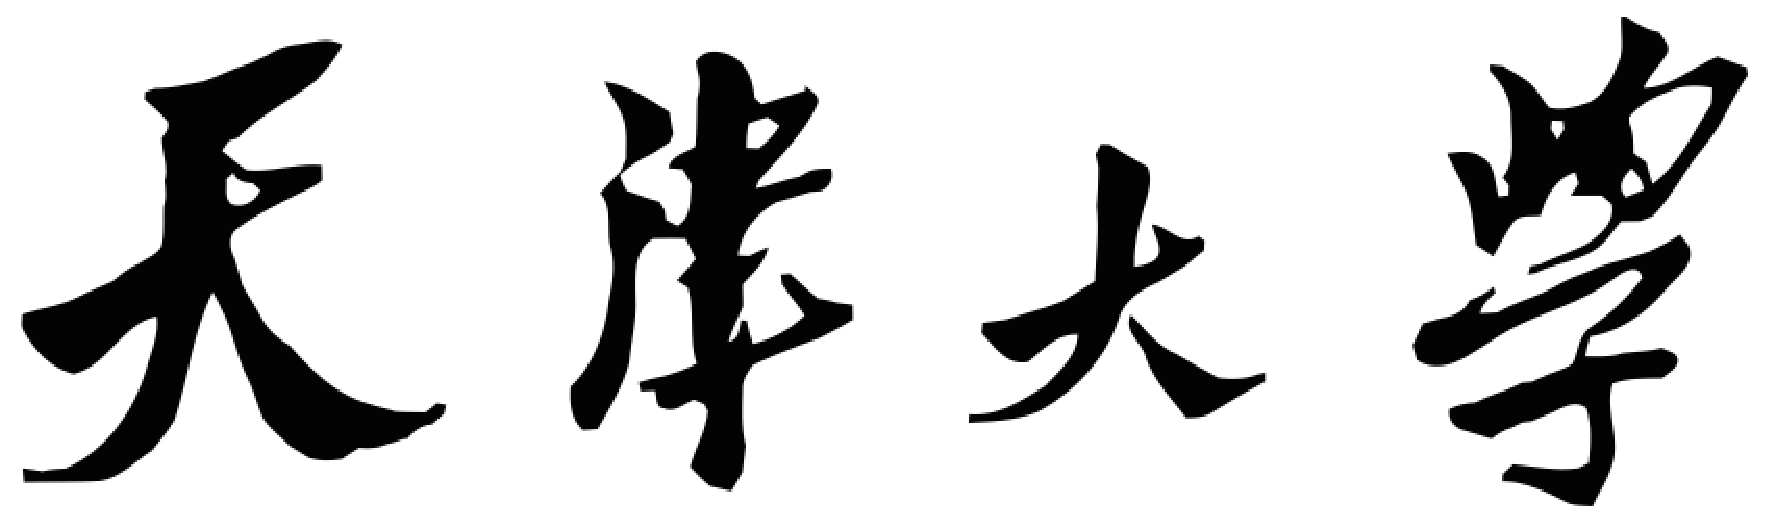
\includegraphics[width=0.4\textwidth]{figures/tjuname.eps}
  \end{figure}
  \vspace*{15pt}
  \hei\erhao{\textbf{本科生毕业论文}}
  \vspace*{72.5pt}

  \begin{figure}[h]
  \centering
  
\includegraphics[width=0.3\textwidth]{figures/tjulogo.eps}
  \end{figure}

  \vspace*{5pt}
  \hei\sanhao{\textbf{题目:\@ctitle}}
  \vspace*{16pt}
  
  \vspace*{24pt}
  \renewcommand\arraystretch{1.5}
  \setlength{\@title@width}{5cm}
  {\sanhao\song{\bf{
  \begin{tabular}{lc}
    学\qquad 院&  \underline{\makebox[\@title@width][c]{\@caffil}} \\
    专\qquad 业 &  \underline{\makebox[\@title@width][c]{\@csubject}} \\
    年\qquad 级  &  \underline{\makebox[\@title@width][c]{\@cgrade}}\\
    姓\qquad 名 &  \underline{\makebox[\@title@width][c]{\@cauthor}} \\
    学\qquad 号 &  \underline{\makebox[\@title@width][c]{\@cnumber}} \\
    指导教师 &  \underline{\makebox[\@title@width][c]{\@csupervisor}} \\
  \end{tabular}}}
 }
  \vspace*{21pt}

\song\sanhao{\textbf{\@cdate}}
\end{center}

%%%%%%%%%%%%%%%%%%%  独创性声明 %%%%%%%%%%%%%%%%%%%%%%%%%%%
\clearpage

\markboth{独创性声明}{独创性声明}
\pdfbookmark[0]{独创性声明}{declare}
\vspace{\baselineskip}
\chapter*{\centering\erhao\song \textbf{独创性声明}}
\vspace{\baselineskip}
\begin{spacing}{1.63}
\song\sanhao

本人声明:所呈交的毕业设计(论文),是本人在指导教师指导下,进行研究工作所取得的成果。除文中已经注明引用的内容外,本毕业设计(论文)中不包含任何他人已经发表或撰写过的研究成果。对本毕业设计(论文)所涉及的研究工作做出贡献的其他个人和集体,均已在论文中作了明确的说明。本毕业设计(论文)原创性声明的法律责任由本人承担。

\vspace{\baselineskip}
\vspace{\baselineskip}
\song\sanhao

\rightline{论文作者签名:\@csign}

\rightline{\the\year~年~\the\month~月~\the\day~日}

\vspace{\baselineskip}
\vspace{\baselineskip}

本人声明:本毕业设计(论文)是本人指导学生完成的研究成果,已经审阅过论文的全部内容。

\vspace{\baselineskip}
\vspace{\baselineskip}

\rightline{论文指导教师签名:\@teachersign}

\rightline{\the\year~年~\the\month~月~\the\day~日}
\thispagestyle{empty}
\end{spacing}
\end{titlepage}

%%%%%%%%%%%%%%%%%%%   Abstract and Keywords  %%%%%%%%%%%%%%%%%%%%%%%
\clearpage
\markboth{摘~要}{摘~要}
\pdfbookmark[0]{摘~~要}{cabstract}
%\addcontentsline{toc}{chapter}{摘~要}
%\chapter*{\centering\sanhao\hei\bfseries 摘\qquad 要}
\chapter*{\centering\erhao\song \textbf{摘\qquad 要}}
\song\defaultfont
\@cabstract
\vspace{\baselineskip}

\hangafter=1\hangindent=0pt\noindent
{\song\sihao\textbf{关键词:}} \@ckeywords
% \thispagestyle{empty}

%%%%%%%%%%%%%%%%%%%   English Abstract  %%%%%%%%%%%%%%%%%%%%%%%%%%%%%%
\clearpage
%\phantomsection
\markboth{ABSTRACT}{ABSTRACT}
\pdfbookmark[0]{ABSTRACT}{eabstract}
%\addcontentsline{toc}{chapter}{ABSTRACT}
\chapter*{\centering\erhao{\textbf{ABSTRACT}}}
%\vspace{\baselineskip}
\noindent
\@eabstract
\vspace{\baselineskip}

\hangafter=1\hangindent=0pt\noindent
{\sihao\textbf{KEY WORDS: }} \@ekeywords
% \thispagestyle{empty}
}
\makeatother
                  % 完成对论文各个部分格式的设置
\frontmatter                          % 以下是论文导言部分,包括论文的封面,中英文摘要和中文目录
\fancypagestyle{plain}{
\fancyhf{}
\renewcommand{\headrulewidth}{0 pt}
\fancyfoot[C]{\song\xiaowu~\thepage~}
}
% \setlength{\voffset}{-12.5mm}  
%%%%%%%%%%   封面 摘要   %%%%%%%%%%
% !Mode:: "TeX:UTF-8"

%%  可通过增加或减少 setup/format.tex中的
%%  第274行 \setlength{\@title@width}{8cm}中 8cm 这个参数来 控制封面中下划线的长度。

\cheading{天津大学~2024~届本科生毕业论文}      % 设置正文的页眉,需要填上对应的毕业年份
\ctitle{春江花月夜}    % 封面用论文标题,自己可手动断行
\caffil{智能与计算学部} % 学院名称
\csubject{软件工程}   % 专业名称
\cgrade{2020~级}            % 年级
\cauthor{张若虚}            % 学生姓名
\cnumber{zhangruoxu111}        % 学生学号
\csupervisor{自学成才}        % 导师姓名

\csign{\quad \quad \quad \quad \quad \quad \quad \quad}

\teachersign{\quad \quad \quad \quad \quad \quad \quad \quad}

% \cdate{\the\year~年~\the\month~月~\the\day~日}



\setcounter{page}{1}                           % 单独从 1 开始编页码
\pagenumbering{Roman}
\thispagestyle{plain}

\cabstract{
《春江花月夜》是唐代诗人张若虚创作的七言歌行。此诗沿用陈隋乐府旧题,运用富有生活气息的清丽之笔,以江为场景,以月为主体,描绘了一幅幽美邈远、惝恍迷离的春江月夜图,抒写了游子思妇真挚动人的离情别绪以及富有哲理意味的人生感慨,突破了梁陈宫体诗的狭小天地,表现了一种迥绝的宇宙意识,创造了一个深沉、寥廓、宁静的艺术境界。

全诗共三十六句,每四句一换韵,通篇融诗情、画意、哲理为一体,意境空明,想象奇特,语言自然隽永,韵律宛转悠扬,为历代文人墨客吟咏唱诵,被闻一多誉为“诗中的诗,顶峰上的顶峰”。
}

\ckeywords{春江花月夜,唐诗,张若虚,七言歌行,游子思乡,离情别绪,唐代艺术文学赏析}

\eabstract{
A Night of Flowers and Moonlight in Spring is a seven-character song line created by Zhang Ruoxu, a poet in Tang Dynasty. This poem follows the old title of Chen Sui's Yuefu, uses a fresh and beautiful brush full of life, takes the river as the scene, takes the moon as the main body, describes a beautiful and distant spring moonlight picture, expresses the sincere and moving parting feelings of the wandering son and the thinking woman and the philosophical feelings of life, breaks through the narrow world of Liang Chen's palace poetry, and expresses a unique cosmic consciousness. Create a deep, boundless, quiet artistic realm.

The poem is composed of thirty-six sentences, every four sentences change rhyme, and the whole poem, painting and philosophy are integrated into one. The artistic conception is clear, the imagination is strange, the language is natural and meaningful, and the rhythm is melodious. It is recited and recited by scholars of all ages, and is praised by Wen Yiduo as "the poem in the poem, the peak on the peak".
}

\ekeywords{Keyword 1, Keyword 2, Keyword 3, Keyword 1, Keyword 2, Keyword 3, Keyword 1, Keyword 2, Keyword 3, }

\makecover

\clearpage
                                % 封面

%%%%%%%%%%   目录   %%%%%%%%%%
\defaultfont
\clearpage{\pagestyle{empty}\cleardoublepage}

\titleformat{\chapter}{\centering\sanhao\hei}{\chaptername}{1em}{} % 设置目录两字的格式
\pdfbookmark[0]{目~~录}{mulu}
\tableofcontents                                     % 中文目录
\fancypagestyle{plain}{
\fancyhf{}
\renewcommand{\headrulewidth}{0 pt}
\fancyfoot[C]{\song\xiaowu~\thepage~}
}
\thispagestyle{plain}

\mainmatter\defaultfont\sloppy\raggedbottom
\makeatletter
\fancypagestyle{plain}{                              % 设置开章页眉页脚风格
    \fancyhf{}
    \fancyhead[C]{\song\wuhao \@cheading}            % 首页页眉格式
    \fancyfoot[C]{\song\xiaowu ~\thepage~}           % 首页页脚格式
    \renewcommand{\headrulewidth}{0.5pt}
    \renewcommand{\footrulewidth}{0pt}
}
\makeatother

\titleformat{\chapter}{\centering\xiaosan\hei}{\chaptername}{1em}{} % 恢复chapter标题格式要求
\setcounter{page}{1}                                 % 单独从 1 开始编页码
\pagenumbering{arabic}
%%%%%%%%%  正文  %%%%%%%%%
% \include{body}
    \chapter{春江潮水连海平}
春江潮水连海平,海上明月共潮生。
滟滟随波千万里,何处春江无月明!
江流宛转绕芳甸,月照花林皆似霰;
空里流霜不觉飞,汀上白沙看不见。
江天一色无纤尘,皎皎空中孤月轮。
江畔何人初见月?江月何年初照人?

甲乙丙丁戊己庚辛壬癸甲乙丙丁戊己庚辛壬癸甲乙丙丁戊己庚辛壬癸甲乙丙丁戊

\section{床前明月光}
% 床前明月光
\subsection{疑是地上霜}
疑是地上霜

\section{床前明月光}
\subsection{疑是地上霜}
疑是地上霜

\begin{figure}[htbp]
\centering

\includegraphics[width=0.4\textwidth]{Thesis/figures/tjulogo.eps}
\caption{Welcom to TJU!}
\end{figure}

    \chapter{理论研究}
此处格式已按模板设定,作者只需选择段落区域,输入替换之。模版中所有说明性文字用于注释格式与内容的要求,撰写论文时请删除。模版中,图表、公式、参考文献等都已给出范例,撰写论文时请删除。

本模版已包含符合章节设置的“多级别列表”,只需在相应位置替换标题文字即可。如需增加章节,建议先使用格式刷,再调整编号。

\section{结构及要求}
\subsection{论文结构}
毕业设计(论文)原则上应采用中文完成(教学语言为英语的除外),确需用其他语言撰写的需经学院审批同意并报教务处备案。毕业设计(论文)一般由以下部分组成,依次为:①封面;②扉页;③独创性声明;④中英文摘要及关键词;⑤目录;⑥正文;⑦参考文献;⑧附录;⑨致谢。

\subsection{语言表述}
要做到数据可靠、推理严谨、立论正确。论述必须简明扼要、重点突出,对同行专业人员已熟知的常识性内容,尽量减少叙述。

论文中如出现一些非通用性的新名词、术语或概念,需做出解释。

\subsection{标题和层次}
标题要重点突出,简明扼要,层次要清楚。

\subsection{打印规格}
论文一律采用A4纸张(大小为210mm×297mm)打印,可根据实际选择单面或双面印刷,页边距如下设置。上:27.5mm;下:25.4mm;左:35.7mm;右:27.7mm。页眉距边界15.0mm;页脚距边界17.5mm。字符间距为默认值(缩放100%,间距:标准)。

\section{论文撰写规范}

\subsection{封面}
采用天津大学本科生毕业设计(论文)统一封面,封面内容包括论文题目、学院、专业、年级、姓名、学号、指导教师等信息。

论文题目是论文总体内容的体现,要求醒目、简明、准确,主题突出,一般不宜超过25字。

\subsection{目录}
目录的各章节应简明扼要,应列至三级标题,包含正文及其后的各部分,并附有相应页码。目录的文字应与相应标题文字完全一致。

“目录”两字之间空一个全角空格或两个半角空格,采用不编号章标题样式。目录条目采用正文样式。

各级标题采用逐级缩进形式,每级缩进2字符,页码前导符采用“…”。

\subsection{正文}
正文是毕业设计(论文)的主体,应占据主要篇幅,文字一般不少于15000字,要求主题明确,内容充实;论点正确,论据可靠,论证充分。内容一般包括:设计(论文)的工作目的(背景),国内外研究现状、理论分析、计算方法、实验装置和测试方法、实验结果分析与讨论、研究成果、结论及意义等。

正文中文字体为宋体,英文字体为Times New Roman,正文采用小四号字,段落行间距为固定值20磅,段落前后间距为0,首行缩进2字符。西文字体以Times New Roman为准,若Times New Roman中没有相应字符,则应使用较为清晰和通用的字体。数学公式和专门文字(如计算机程序代码)的字体可以根据需要选择。

章节与标号:一般分为章标题(一级标题)、不编号章标题(同属于一级标题)、二级标题和三级标题。各章节编号建议采用Word的“多级别列表”方式自动形成编号,标题编号与标题内容之间空一个全角空格或两个半角空格。各级章节标题格式要求细节参见《天津大学本科生毕业设计(论文)撰写规范》。

图、表等与其前后的正文之间要有一行的间距;文中的图、表、公式一律采用阿拉伯数字分章编号,如:图2-5,表3-2,公式(5-1)(“公式”两个字不要写上)等。若图或表中有附注,采用英文小写字母顺序编号。子图采用英文字母编号。引用图或表应在图题或表题右上角标出文献来源。图或表的附注应位于图或表的下方。


%%%%%%%%%%  参考文献  %%%%%%%%%%
\defaultfont
\bibliographystyle{references/ref.buk}
\phantomsection
\markboth{参考文献}{参考文献}
\addcontentsline{toc}{chapter}{参考文献}       % 参考文献加入到中文目录
% \nocite{*}        % 若将此命令屏蔽掉,则未引用的文献不会出现在文后的参考文献中
\bibliography{references/reference}

\titleformat{\chapter}{\centering\xiaosan\hei}{\chaptername}{1em}{}

% % !Mode:: "TeX:UTF-8"

\titlecontents{chapter}[2em]{\vspace{.5\baselineskip}\xiaosan\song}%
             {\prechaptername\CJKnumber{\thecontentslabel}\postchaptername\qquad}{} %
             {}             % 设置该选项为空是为了不让目录中显示页码
\addcontentsline{toc}{chapter}{外文资料}
%\setcounter{page}{1}       % 如果需要从该页开始从 1 开始编页,则取消该注释
\markboth{外文资料}{外文资料}
\chapter*{外文资料}

Here follows the English paper.

...              % 外文资料
% % !Mode:: "TeX:UTF-8"

\titlecontents{chapter}[2em]{\vspace{.5\baselineskip}\xiaosan\song}
             {\prechaptername\CJKnumber{\thecontentslabel}\postchaptername\qquad}{}
             {}             % 设置该选项为空是为了不让目录中显示页码
\addcontentsline{toc}{chapter}{中文译文}
\setcounter{page}{1}            % 单独从 1 开始编页码
\markboth{中文译文}{中文译文}   % 用于将章节号添加到页眉中
\chapter*{中文译文}

这里就是外文资料的中文翻译。

...
              % 中文译文
% !Mode:: "TeX:UTF-8"

% \titlecontents{chapter}[2em]{\vspace{.5\baselineskip}\xiaosan\song} {\prechaptername\CJKnumber{\thecontentslabel}\postchaptername\qquad}{}{}                            % 设置该选项为空是为了不让目录中显示页码
% \fancypagestyle{plain}   % 设置页眉页脚风格
\lhead{}
\rhead{}
\chead{\song\wuhao 天津大学 2024 届本科生毕业论文} % 设置页眉内容
\lfoot{}
\cfoot{}
\rfoot{}
\markboth{致\quad 谢}{致\quad 谢}
\addcontentsline{toc}{chapter}{致\quad 谢} % 添加到目录中
\chapter*{\hei\xiaosan 致\quad 谢}
% \setcounter{page}{1}

谢谢春江花月夜。            % 致谢

\clearpage
\end{document}                                 % 结束全文
